% Trying to break the document up a bit.  This command simply inserts the contents of the file at this point.  It contains the document license, preamble, and title page: things that aren't likely to change more than once.  This can be used to separate discrete parts of a document into files that are easier to edit at one time.
%%%%%%%%%%%%%%%%%%%%%%%%%%%%%%%%%%%%%%%%%%%%%%%%%%%%%%%%%%%%%%%%%%%%%%
% This layout was adapted from one found at latextemplates.com which
% was adapted from another.
%
% License: CC BY-NC-SA 3.0
% (http://creativecommons.org/licenses/by-nc-sa/3.0/)
%
% Original header:
%
% This is a LaTeX version of the sample laboratory report from
% Virginia Tech's copyrighted 08-09 CHEM 1045/1046 lab manual.
% Reproduction of this one appendix section for academic purposes
% should fall under fair use.
%
%%%%%%%%%%%%%%%%%%%%%%%%%%%%%%%%%%%%%%%%%%%%%%%%%%%%%%%%%%%%%%%%%%%%%%

\documentclass{article}

\usepackage{graphicx}
% \usepackage[acronym]{glossaries} % Lets us use acronyms
\usepackage{multicol}
\usepackage{amsmath}
\usepackage{siunitx} % SI units in math mode
\usepackage{subcaption}

\author{}
\title{ELEC-313 \\ Lab 5: CMOS Circuits\\ }
\date{\today}

% \loadglsentries{acronyms} % Actually loads 'acronyms.tex'
% \makeglossaries

\begin{document}

\maketitle

\begin{center}
  \begin{tabular}{lr}
    Date Performed: & October 16, 2013 \\
    Partners:       & Charles Pittman    \\
    & Stephen Wilson     \\
  \end{tabular}
\end{center}

\newpage

\tableofcontents
\listoffigures
\listoftables
\newpage

% Number the enumerate environment (unordered lists) by letter:
\renewcommand{\labelenumi}{\alph{enumi}.}

\section{Objective}

\section{Equipment}

\begin{tabular}{ll}
  \centering
  Transistor: 2N2222A               & Power supply: HP E3631A            \\
  Resistors: \SI{22}{\kilo\ohm}, \SI{33}{\kilo\ohm}, \SI{220}{\ohm} (x2) &   Capacitor: \SI{0.1}{\micro\farad} \\
 Multimeters: HP 34401A, Fluke 8010A (x2) & \\
\end{tabular}

\section{Schematics}

% \begin{figure}[hbtp]
%   \centering
%   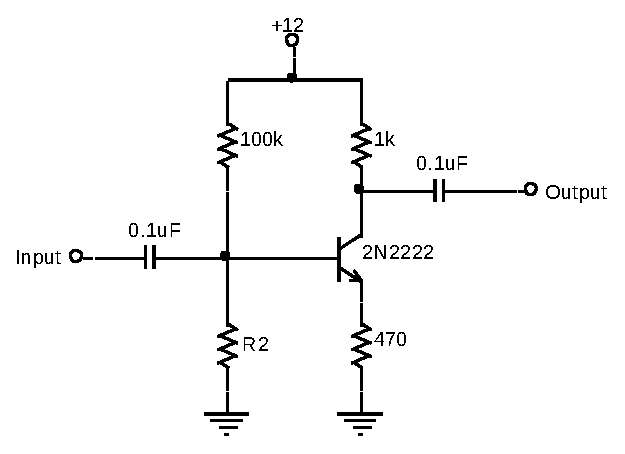
\includegraphics[width=0.6\textwidth]{circuit}
%   \caption{\label{fig:circuit} Common-emitter transistor circuit}
% \end{figure}

% \begin{figure}[hbtp]
%   \centering
%   \begin{subfigure}[b]{0.5\textwidth}
%     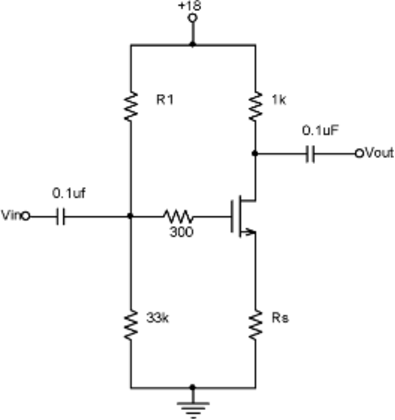
\includegraphics[width=\textwidth]{common-source}
%     \caption{\label{schem:common-source} Common-source amplifier}
%   \end{subfigure}%
%   ~
%   \begin{subfigure}[b]{0.5\textwidth}
%     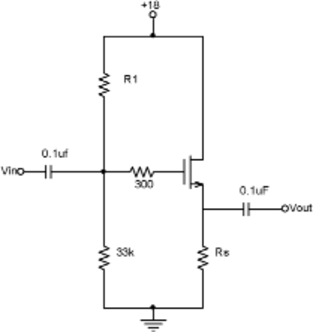
\includegraphics[width=\textwidth]{source-follower}
%     \caption{\label{schem:source-follower} Source-follower amplifier}
%   \end{subfigure}
%   \caption{\label{fig:schematics} Circuits used in this lab. $R_1=\SI{100}{\kilo\ohm}$,  $R_s=\SI{470}{\ohm}$}
% \end{figure}

\section{Procedure}

\section{Results}

% \begin{table}[hbtp]
%   \centering
%   \begin{tabular}{cccc}
%     $V_{CC}$ & $I_C$     & $V_{CE}$ & $\beta$ \\
%     (\si{V}) & (\si{mA}) & (\si{V}) &         \\
%     \hline
%     0.50     & 0.232     & 0.454    & 11.60   \\
%     0.75     & 0.233     & 0.705    & 11.65   \\
%     1.00     & 0.234     & 0.954    & 11.70   \\
%     1.25     & 0.237     & 1.204    & 11.85   \\
%     1.50     & 0.237     & 1.454    & 11.85   \\
%     2        & 0.242     & 1.954    & 12.10   \\
%     4        & 0.25      & 3.95     & 12.30   \\
%     6        & 0.25      & 5.95     & 12.60   \\
%     8        & 0.26      & 7.95     & 12.75   \\
%     10       & 0.26      & 9.96     & 12.85   \\
%     12       & 0.26      & 11.95    & 13.10   \\
%     14       & 0.27      & 13.94    & 13.30   \\
%     16       & 0.27      & 15.95    & 13.40   \\
%     18       & 0.27      & 17.95    & 13.50   \\
%     20       & 0.27      & 19.95    & 13.70   \\
%   \end{tabular}
%   \caption{\label{tab:1} $I_B = $ \SI{20}{\micro\ampere}}
% \end{table}

% \begin{table}[hbtp]
%   \centering
%   \begin{tabular}{cc}
%     $I_B$ (\si{\micro\ampere}) & $\beta_{avg}$ \\
%     \hline
%     20                         & 12.55         \\
%     50                         & 105.85        \\
%     80                         & 132.00        \\
%     100                        & 137.99        \\
%   \end{tabular}
%   \caption{\label{tab:beta_IB} Average values of $\beta$ per $I_B$}
% \end{table}

% \begin{figure}[hbtp]
%   \centering
%   \resizebox{1.0\textwidth}{!}{% GNUPLOT: LaTeX picture with Postscript
\begingroup
  \makeatletter
  \providecommand\color[2][]{%
    \GenericError{(gnuplot) \space\space\space\@spaces}{%
      Package color not loaded in conjunction with
      terminal option `colourtext'%
    }{See the gnuplot documentation for explanation.%
    }{Either use 'blacktext' in gnuplot or load the package
      color.sty in LaTeX.}%
    \renewcommand\color[2][]{}%
  }%
  \providecommand\includegraphics[2][]{%
    \GenericError{(gnuplot) \space\space\space\@spaces}{%
      Package graphicx or graphics not loaded%
    }{See the gnuplot documentation for explanation.%
    }{The gnuplot epslatex terminal needs graphicx.sty or graphics.sty.}%
    \renewcommand\includegraphics[2][]{}%
  }%
  \providecommand\rotatebox[2]{#2}%
  \@ifundefined{ifGPcolor}{%
    \newif\ifGPcolor
    \GPcolortrue
  }{}%
  \@ifundefined{ifGPblacktext}{%
    \newif\ifGPblacktext
    \GPblacktextfalse
  }{}%
  % define a \g@addto@macro without @ in the name:
  \let\gplgaddtomacro\g@addto@macro
  % define empty templates for all commands taking text:
  \gdef\gplbacktext{}%
  \gdef\gplfronttext{}%
  \makeatother
  \ifGPblacktext
    % no textcolor at all
    \def\colorrgb#1{}%
    \def\colorgray#1{}%
  \else
    % gray or color?
    \ifGPcolor
      \def\colorrgb#1{\color[rgb]{#1}}%
      \def\colorgray#1{\color[gray]{#1}}%
      \expandafter\def\csname LTw\endcsname{\color{white}}%
      \expandafter\def\csname LTb\endcsname{\color{black}}%
      \expandafter\def\csname LTa\endcsname{\color{black}}%
      \expandafter\def\csname LT0\endcsname{\color[rgb]{1,0,0}}%
      \expandafter\def\csname LT1\endcsname{\color[rgb]{0,1,0}}%
      \expandafter\def\csname LT2\endcsname{\color[rgb]{0,0,1}}%
      \expandafter\def\csname LT3\endcsname{\color[rgb]{1,0,1}}%
      \expandafter\def\csname LT4\endcsname{\color[rgb]{0,1,1}}%
      \expandafter\def\csname LT5\endcsname{\color[rgb]{1,1,0}}%
      \expandafter\def\csname LT6\endcsname{\color[rgb]{0,0,0}}%
      \expandafter\def\csname LT7\endcsname{\color[rgb]{1,0.3,0}}%
      \expandafter\def\csname LT8\endcsname{\color[rgb]{0.5,0.5,0.5}}%
    \else
      % gray
      \def\colorrgb#1{\color{black}}%
      \def\colorgray#1{\color[gray]{#1}}%
      \expandafter\def\csname LTw\endcsname{\color{white}}%
      \expandafter\def\csname LTb\endcsname{\color{black}}%
      \expandafter\def\csname LTa\endcsname{\color{black}}%
      \expandafter\def\csname LT0\endcsname{\color{black}}%
      \expandafter\def\csname LT1\endcsname{\color{black}}%
      \expandafter\def\csname LT2\endcsname{\color{black}}%
      \expandafter\def\csname LT3\endcsname{\color{black}}%
      \expandafter\def\csname LT4\endcsname{\color{black}}%
      \expandafter\def\csname LT5\endcsname{\color{black}}%
      \expandafter\def\csname LT6\endcsname{\color{black}}%
      \expandafter\def\csname LT7\endcsname{\color{black}}%
      \expandafter\def\csname LT8\endcsname{\color{black}}%
    \fi
  \fi
  \setlength{\unitlength}{0.0500bp}%
  \begin{picture}(7200.00,5040.00)%
    \gplgaddtomacro\gplbacktext{%
      \csname LTb\endcsname%
      \put(726,440){\makebox(0,0)[r]{\strut{}0mA}}%
      \csname LTb\endcsname%
      \put(726,1307){\makebox(0,0)[r]{\strut{}5mA}}%
      \csname LTb\endcsname%
      \put(726,2174){\makebox(0,0)[r]{\strut{}10mA}}%
      \csname LTb\endcsname%
      \put(726,3041){\makebox(0,0)[r]{\strut{}15mA}}%
      \csname LTb\endcsname%
      \put(726,3908){\makebox(0,0)[r]{\strut{}20mA}}%
      \csname LTb\endcsname%
      \put(726,4775){\makebox(0,0)[r]{\strut{}25mA}}%
      \csname LTb\endcsname%
      \put(858,220){\makebox(0,0){\strut{}0 V}}%
      \csname LTb\endcsname%
      \put(1453,220){\makebox(0,0){\strut{}2 V}}%
      \csname LTb\endcsname%
      \put(2047,220){\makebox(0,0){\strut{}4 V}}%
      \csname LTb\endcsname%
      \put(2642,220){\makebox(0,0){\strut{}6 V}}%
      \csname LTb\endcsname%
      \put(3236,220){\makebox(0,0){\strut{}8 V}}%
      \csname LTb\endcsname%
      \put(3831,220){\makebox(0,0){\strut{}10 V}}%
      \csname LTb\endcsname%
      \put(4425,220){\makebox(0,0){\strut{}12 V}}%
      \csname LTb\endcsname%
      \put(5020,220){\makebox(0,0){\strut{}14 V}}%
      \csname LTb\endcsname%
      \put(5614,220){\makebox(0,0){\strut{}16 V}}%
      \csname LTb\endcsname%
      \put(6209,220){\makebox(0,0){\strut{}18 V}}%
      \csname LTb\endcsname%
      \put(6803,220){\makebox(0,0){\strut{}20 V}}%
    }%
    \gplgaddtomacro\gplfronttext{%
      \csname LTb\endcsname%
      \put(5816,4602){\makebox(0,0)[r]{\strut{}$I_B = $SI{20}{microampere}}}%
      \csname LTb\endcsname%
      \put(5816,4382){\makebox(0,0)[r]{\strut{}$I_B = $SI{50}{microampere}}}%
      \csname LTb\endcsname%
      \put(5816,4162){\makebox(0,0)[r]{\strut{}$I_B = $SI{80}{microampere}}}%
      \csname LTb\endcsname%
      \put(5816,3942){\makebox(0,0)[r]{\strut{}$I_B = $SI{100}{microampere}}}%
    }%
    \gplbacktext
    \put(0,0){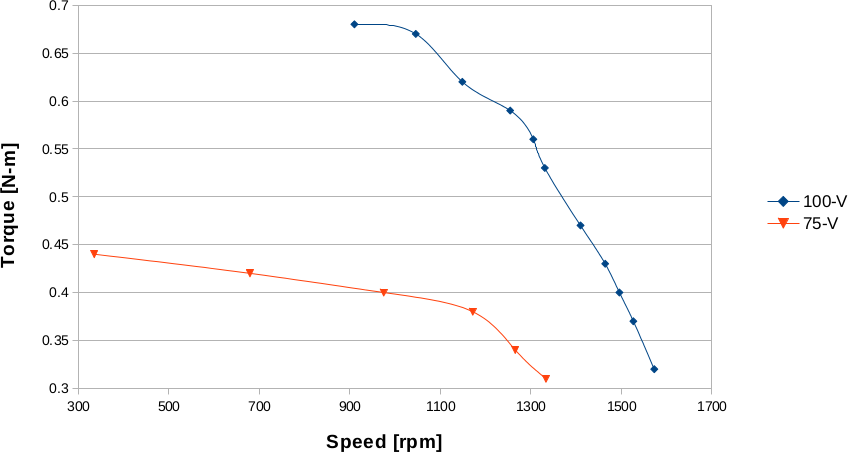
\includegraphics{graph}}%
    \gplfronttext
  \end{picture}%
\endgroup
}
%   \caption{\label{fig:graph} $V_{CE}$ vs. $I_C$}
% \end{figure}

\newpage
\section{Conclusion}
\label{sec:conclusion}

\section{Equations}

% LaTeX sees blank lines as a start of another paragraph.  To avoid
% unnecessary vertical spaces between equations, and still visually
% separate in source, put a comment between them.
%
% \begin{equation}
%   \label{eq:beta}
%   \beta = \frac{I_C}{I_B}
% \end{equation}
% %
% \begin{equation}
%   \label{eq:hoe}
%   h_{oe} \approx \frac{1}{r_o} = \frac{\Delta I_C}{\Delta V_{CE}}
% \end{equation}
%
% \begin{equation}
%   \label{eqn:percent_diff}
%   \%_{diff} = \frac{|measured - theoretical|}{theoretical} \times 100\%
% \end{equation}

\end{document}
